
\documentclass[12pt, a4paper]{article}

%-----------USEPACKAGE----------------------------
\usepackage{bm} % Tucne pismo
\usepackage[czech]{babel} % Cestina
\usepackage[T1]{fontenc}
\usepackage[utf8x]{inputenc}
\linespread{1.10} % Radkovani 1.3 odpovida radkovani 2
\usepackage{lmodern} % Daji se pouzit \HUGE atd.
\usepackage{amsmath}
\usepackage{algorithm}
\usepackage[noend]{algpseudocode} % Vkladani pseudo kodu
\usepackage{listings}
\usepackage{setspace}

% Graphics
\usepackage{graphicx}
\usepackage{epstopdf}
\usepackage{color}
\graphicspath{{./img/}}

% Hyperref and its color
\usepackage[unicode]{hyperref} % Odkazy v pdf, www a na e-mail
\usepackage[hypcap=true]{caption}
\usepackage[hypcap=true,list=true]{subcaption}
\hypersetup{colorlinks = true, citecolor = black}
\hypersetup{linkcolor=red}
\hypersetup{colorlinks,urlcolor=black}








%-----------COLORS--------------------------------
\definecolor{Code}{rgb}{0,0,0}
\definecolor{Decorators}{rgb}{0.5,0.5,0.5}
\definecolor{Numbers}{rgb}{0.5,0,0}
\definecolor{MatchingBrackets}{rgb}{0.25,0.5,0.5}
\definecolor{Keywords}{rgb}{0,0,1}
\definecolor{self}{rgb}{0,0,0}
\definecolor{Strings}{rgb}{0,0.63,0}
\definecolor{Comments}{rgb}{0,0.63,1}
\definecolor{Backquotes}{rgb}{0,0,0}
\definecolor{Classname}{rgb}{0,0,0}
\definecolor{FunctionName}{rgb}{0,0,0}
\definecolor{Operators}{rgb}{0,0,0}
\definecolor{Background}{rgb}{1, 1, 1}

%-----------LISTINGS-SETTINGS----------------------
\lstset{
	numbers=left,
	numberstyle=\footnotesize,
	numbersep=0.5em,
	xleftmargin=1.5em,
	xrightmargin=0em,
	framextopmargin=0em,
	framexbottommargin=0em,
	showspaces=false,
	showtabs=false,
	showstringspaces=false,
	frame=lrtb,
	tabsize=4,
	% Basic
	basicstyle=\ttfamily\footnotesize\setstretch{1},
	backgroundcolor=\color{Background},
	language=Python,
	% Comments
	commentstyle=\color{Comments}\slshape,
	% Strings
	stringstyle=\color{Strings},
	morecomment=[s][\color{Strings}]{"""}{"""},
	morecomment=[s][\color{Strings}]{'''}{'''},
	% Keywords
morekeywords={import,from,class,def,for,while,if,is,in,elif,else,not,and,or,print,break,continue,return,True,False,None,access,as,del,except,exec,finally,global,import,lambda,pass,print,raise,try,assert},
	keywordstyle={\color{Keywords}\bfseries},
	% Additional keywords
	morekeywords={[2]@invariant},
	keywordstyle={[2]\color{Decorators}\slshape},
	emph={self},
	emphstyle={\color{self}\slshape},
	breaklines=true, % Zalamuje radky.
}






%------------------VARIABLES----------------------------
\newcommand{\cisloCviceni}{5. cvičení}









%------------------LAYOUT----------------------------
\usepackage[top = 2.5 cm, bottom = 2.5 cm, left = 2.5 cm, right = 2.5 cm]{geometry} % geometrie stranky
\usepackage{longtable}% Pro dlouhy obsah, da se zalomit \pagebrek
\usepackage{fancyhdr}
\pagestyle{fancy}% Deffaultni nastaveni hlavicky a paticky
\setlength{\headheight}{16 pt}% Zvetsi hlavicku, aby to nedelalo warningy
\fancyhf{}
\lhead{\href{http://www.kky.zcu.cz/cs/courses/mpv}{Metody Počítačového Vidění}}
\rhead{\cisloCviceni}
\fancyfoot[R]{\thepage}
\fancyfoot[L]{Verze 2.0.0, poslední úpravy: \today}








%---------------BEGIN-DOCUMENT--------------------------
\begin{document}
 









 
%--------TITLE-PAGE--------------------------------------------
\begin{titlepage}
\begin{center}
	
\includegraphics[trim = 0.6cm 0.5cm 0.9cm 0.5cm, scale=1]{./FAV_logo_cz.pdf}
	\hspace*{\fill}
	
\includegraphics[trim = 3.5cm 1.5cm 2.6cm 2cm, scale=0.295]{./KKY_logo_cz.pdf}\\
	\vspace*{\fill}
	\textbf{\Huge{\href{http://www.kky.zcu.cz/cs/courses/mpv}{Metody Počítačového Vidění} \\ ~ \\ \cisloCviceni}}\\
	\vspace*{\fill}
	\textbf{\large{\href{mailto:LBures@kky.zcu.cz}{Ing. Lukáš Bureš}}} \hfill \textbf{\large{Plzeň, \today}}
\end{center}
\end{titlepage}












%--------OBSAH-CVICENI---------------------------------
\section*{Obsah cvičení}
\begin{enumerate}
	\item Lokální binární vzor (Local Binary Pattern - LBP)
\end{enumerate}



%--------LBP-----------------------------------------------------------------------
\section{Lokální binární vzor (Local Binary Pattern - LBP)}
\par{Metoda lokálních binárních vzorů (Local Binary Pattern - LBP) je metoda pro popis textury (obrázku) na základě příznaku, který obraz charakterizuje. V případě LBP je příznak reprezentován histogramem.}

\subsubsection*{Implementace základního algoritmu LBP}
\par{Nyní bude stručně nastíněn základní princip LBP, který bude Vaším úkolem implementovat na cvičení:}
\begin{enumerate}
	\item Načíst barevný obrázek s texturou $I$.
	\item Převést $I$ do odstínů šedi na $I_{GS}$.
	\item Rozdělit načtenou texturu, která má velikost $512 \times 512$ pixelů, na buňky $C_{ij}$ o~velikosti $128 \times 128$ pixelů.
	\item Pro každý nehraniční pixel $p_{xy}$ v buňce $C_{ij}$ vypočítat LBP kód. Pokud $p_{xy} > p_{okoli} \rightarrow 1$, jinak $0$. MSB je v levý horní pixel a pokračuj po směru hodinových ručiček až k~LSB.
		\begin{figure}[!ht]
			\centering
			%trim option's parameter order: left bottom right top
			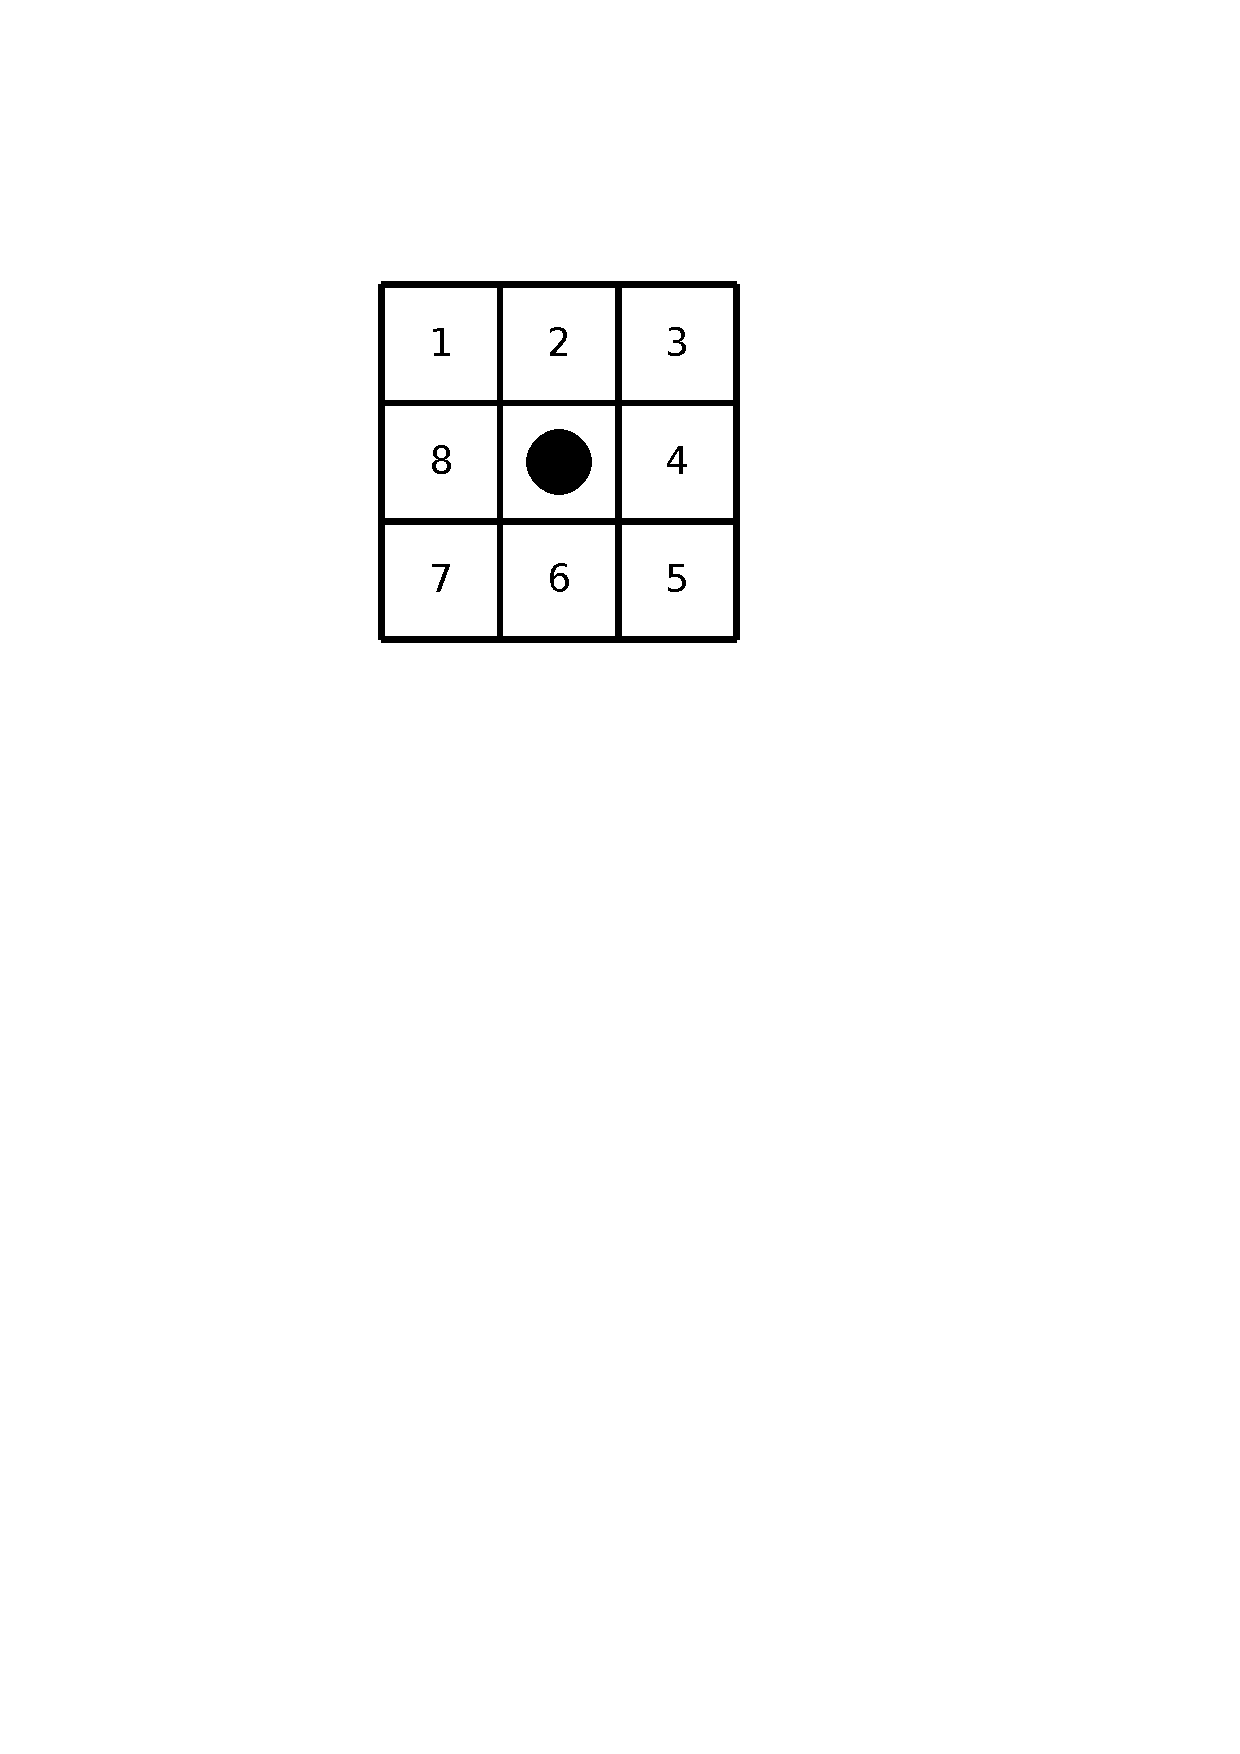
\includegraphics[width = 0.4\textwidth, trim = 4cm 19cm 5cm 4.5cm]{./okoli.pdf}
			\caption{Směr procházení okolí.}
		\end{figure}
	\item Získaný binární kód převeď do dekadické soustavy a vypočti histogram ze všech kódů v~buňce.
	\item Histogram znormuj.
	\item Řetěz jednotlivé histogramy do vektoru o velikosti $256 \cdot 16 = 4096$.
	\item Znormuj zřetězené histogramy.
\end{enumerate}




\newpage


\subsubsection*{Porovnávání histogramů}
\par{Implementujte následující metody porovnávání histogramů:
\begin{enumerate}
	\item Euklidovská vzdálenost: 
		\begin{equation}
			D_E(\bm{X_1}, \bm{X_2}) = \sum \sqrt{\left( \bm{X_1} - \bm{X_2} \right)^{2}}.
		\end{equation}
	\item Chi-square vzdálenost:
		\begin{equation}
			D_{Chi^2}(\bm{X_1}, \bm{X_2}) = \sum \frac{\left( \bm{X_1} - \bm{X_2} \right)^{2}}{\bm{X_1}}.
		\end{equation}
	\item Histogram intersection:
		\begin{equation}
			D_{HI}(\bm{X_1}, \bm{X_2}) = 1 - \sum \min \left( \bm{X_1}, \bm{X_2} \right).
		\end{equation}
	\item 
		\begin{equation}
			D_{4}(\bm{X_1}, \bm{X_2}) = \sum \bm{X_2} \log \left( \frac{\bm{X_2}}{\bm{X_1}} \right)
		\end{equation}
\end{enumerate}}





\subsubsection*{Příklady okolí pro výpočet LBP}
\begin{figure}[!ht]
	\centering
	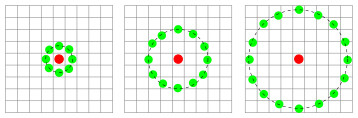
\includegraphics[width = 0.6\textwidth]{./Lbp_neighbors.jpg}
	\caption{Tři příklady okolí pro výpočet lokálního binárního vzoru.}
\end{figure}




\end{document}



















